% Auto-generated by experiments.analysis.generate_win_counts --slides --- do not edit.
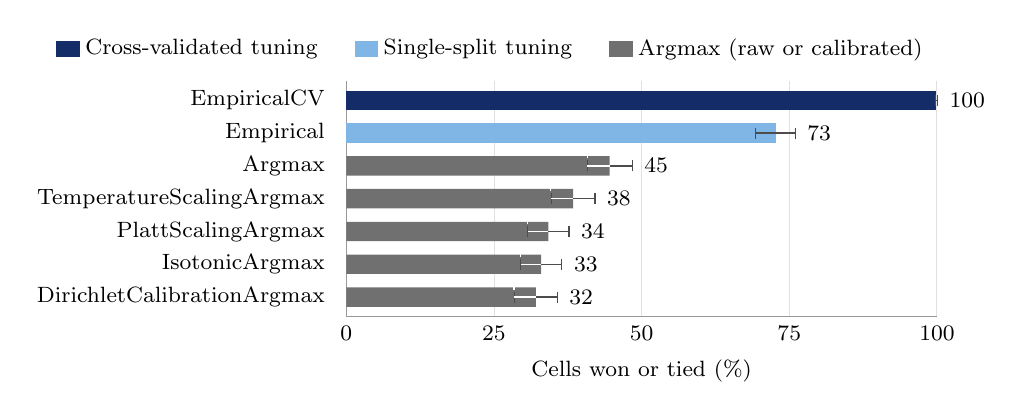
\begin{tikzpicture}
\definecolor{winbarcv}{HTML}{142D69}
\definecolor{winbarsplit}{HTML}{7FB6E6}
\definecolor{winbaranalytical}{HTML}{E6AF3C}
\definecolor{winbarargmax}{HTML}{707070}
\begin{axis}[
    xbar, bar shift=0pt, bar width=7pt,
    scale only axis, width=7.5cm, height=3.00cm,
    xmin=0, xmax=100, xtick={0,25,50,75,100},
    xlabel={Cells won or tied (\%)},
    ymin=0.4, ymax=7.6, y dir=reverse,
    ytick={1,2,3,4,5,6,7},
    yticklabels={EmpiricalCV,Empirical,Argmax,TemperatureScalingArgmax,PlattScalingArgmax,IsotonicArgmax,DirichletCalibrationArgmax},
    axis x line*=bottom, axis y line*=left,
    axis line style={draw=black!40},
    tick style={draw=none},
    xmajorgrids=true,
    major grid style={draw=black!12, line width=0.3pt},
    tick label style={font=\footnotesize},
    label style={font=\footnotesize},
    clip=false,
    legend columns=3,
    legend cell align=left,
    legend image code/.code={\fill[#1] (0cm,-0.1cm) rectangle (0.3cm,0.1cm);},
    legend style={draw=none, fill=none, font=\footnotesize,
        at={(1,1.04)}, anchor=south east,
        /tikz/every even column/.append style={column sep=0.4cm}},
]
\addplot[fill=winbarcv, draw=none, error bars/x dir=both, error bars/x explicit, error bars/error bar style={black!70, line width=0.5pt}] coordinates { (99.9,1) +- (0.2,0) };
\addlegendentry{Cross-validated tuning}
\addplot[fill=winbarsplit, draw=none, error bars/x dir=both, error bars/x explicit, error bars/error bar style={black!70, line width=0.5pt}] coordinates { (72.7,2) +- (3.4,0) };
\addlegendentry{Single-split tuning}
\addplot[fill=winbarargmax, draw=none, error bars/x dir=both, error bars/x explicit, error bars/error bar style={black!70, line width=0.5pt}] coordinates { (44.6,3) +- (3.8,0) (38.4,4) +- (3.7,0) (34.2,5) +- (3.5,0) (33.0,6) +- (3.5,0) (32.1,7) +- (3.7,0) };
\addlegendentry{Argmax (raw or calibrated)}
\draw[white, line width=0.5pt] (axis cs:44.6,3) -- (axis cs:40.8,3) +(0,-2pt) -- +(0,2pt);
\draw[white, line width=0.5pt] (axis cs:38.4,4) -- (axis cs:34.6,4) +(0,-2pt) -- +(0,2pt);
\draw[white, line width=0.5pt] (axis cs:34.2,5) -- (axis cs:30.7,5) +(0,-2pt) -- +(0,2pt);
\draw[white, line width=0.5pt] (axis cs:33.0,6) -- (axis cs:29.5,6) +(0,-2pt) -- +(0,2pt);
\draw[white, line width=0.5pt] (axis cs:32.1,7) -- (axis cs:28.4,7) +(0,-2pt) -- +(0,2pt);
\node[anchor=west, font=\footnotesize, inner sep=1pt] at (axis cs:101.6,1) {100};
\node[anchor=west, font=\footnotesize, inner sep=1pt] at (axis cs:77.5,2) {73};
\node[anchor=west, font=\footnotesize, inner sep=1pt] at (axis cs:49.9,3) {45};
\node[anchor=west, font=\footnotesize, inner sep=1pt] at (axis cs:43.6,4) {38};
\node[anchor=west, font=\footnotesize, inner sep=1pt] at (axis cs:39.2,5) {34};
\node[anchor=west, font=\footnotesize, inner sep=1pt] at (axis cs:38.0,6) {33};
\node[anchor=west, font=\footnotesize, inner sep=1pt] at (axis cs:37.2,7) {32};
\end{axis}
\end{tikzpicture}%
